% !TEX root = task-1-13-1.tex
% Editable task bank. Append new BankTask blocks at the end of the document.
\documentclass[12pt,a4paper]{article}
\usepackage{physics-textbook}
\usepackage{graphicx,needspace}
\usetikzlibrary{decorations.pathmorphing}
\newif\ifShowSolutions
\ifdefined\TutorEdition
  \ShowSolutionstrue
\else
  \ShowSolutionsfalse % Change to \ShowSolutionstrue to display solutions.
\fi
\newcounter{banktask}
\newsavebox{\BankTaskBox}
\newcommand{\BankTaskContent}[3]{%
  \noindent\textbf{\thebanktask.}\quad #2\par
  \ifShowSolutions
    \Needspace{50mm}% Keep the solution heading with its opening text or diagram.
    #3\par
    \ifdefined\TutorEdition
      \ifcsname TutorSource#1\endcsname
        \nopagebreak\smallskip{\small\csname TutorSource#1\endcsname\par}%
      \fi
    \fi
  \fi
}
\newcommand{\BankTask}[3]{%
  \refstepcounter{banktask}\par\medskip
  \sbox{\BankTaskBox}{\begin{minipage}{\linewidth}%
    \BankTaskContent{#1}{#2}{#3}\end{minipage}}%
  \ifdim\dimexpr\ht\BankTaskBox+\dp\BankTaskBox\relax>\dimexpr\textheight-20mm\relax
    \Needspace{35mm}\BankTaskContent{#1}{#2}{#3}%
  \else
    \Needspace{\dimexpr\ht\BankTaskBox+\dp\BankTaskBox\relax}%
    \noindent\usebox{\BankTaskBox}\par
  \fi
  \medskip
}
\begin{document}
\BookSubsection{1.13.1}{Гидростатическое давление}


% Source sdamgia-46113: https://phys-ege.sdamgia.ru/problem?id=46113
\BankTask{sdamgia-46113}{
Гидростатическое давление, создаваемое водой на горизонтальное дно бассейна без учёта давления атмосферы, равно $25 \,\text{кПа}$. Чему равна глубина бассейна?
}{
\smallskip\noindent\textbf{Решение}\par
Из формулы гидростатического давления $p = \rho gh$ находим глубину бассейна:

$h = \frac{ p}{ \rho g } = \frac{ 25 000}{ 10 \cdot 1000 } = 2{,}5 \,\text{м}.$

Ответ: $2{,}5$.
}

% Source sdamgia-9280: https://phys-ege.sdamgia.ru/problem?id=9280
\BankTask{sdamgia-9280}{
Открытый сосуд с керосином находится при нормальном атмосферном давлении. Определите давление в сосуде на глубине $2$ метра. (Плотность керосина — $800 \,\text{кг/м}^3$, нормальное атмосферное давление примите равным $10^5 \,\text{Па}$.)
}{
\smallskip\noindent\textbf{Решение}\par
Гидростатическое давление в сосуде будет являться суммой атмосферного давления $p_{0}$ и давления столба жидкости высотой $h:$

$p=p_{0} + \rho gh=10 ^{5} + 800 \cdot 10 \cdot 2=116\,\text{кПа}.$

Ответ: $116$.
}

% Source sdamgia-7998: https://phys-ege.sdamgia.ru/problem?id=7998
\BankTask{sdamgia-7998}{
В сосуд высотой $20 \,\text{см}$ налита вода, уровень которой ниже края сосуда на $2 \,\text{см}$. Чему равна сила давления воды на дно сосуда, если площадь дна $0{,}01 \,\text{м}^2$? Атмосферное давление не учитывать. Ускорение свободного падения принять равным $10 \,\text{м}/\,\text{с}^2$.
}{
\smallskip\noindent\textbf{Решение}\par
Сила давления воды равна давлению воды, умноженному на площадь дна. Давление воды равно произведению ускорению свободного падения, плотности и высоты воды. В итоге получаем:

$1000\,\text{кг/м} ^{3} \cdot 10\,\text{м}/\,\text{с} ^{2} \cdot 0{,}18\,\text{м} \cdot 0{,}01\,\text{м} ^{2} = 18\,\text{Н}.$

Ответ: $18$.
 
Примечание.
В вертикальном сосуде сила давления жидкости на дно равна весу жидкости.
}

% Source sdamgia-11547: https://phys-ege.sdamgia.ru/problem?id=11547
\BankTask{sdamgia-11547}{
В сосуд высотой $2 \,\text{м}$ налита некая жидкость, уровень которой ниже края сосуда на $20 \,\text{см}$. Давление жидкости на дно сосуда — $14 \,\text{кПа}$. Определите плотность жидкости. Атмосферное давление не учитывать. Ускорение свободного падения принять равным $10 \,\text{м}/\,\text{с}^2$.
}{
\smallskip\noindent\textbf{Решение}\par
Давление на дно сосуда можно выразить следующей формулой: $p=\rho gh,$ откуда $\rho= \frac{ p}{ gh } ,$ где $h=2\,\text{м} - 0{,}2\,\text{м}=1{,}8\,\text{м}.$ подставим имеющиеся данные:

$\rho= \frac{ 14 \cdot 10 ^{3} \,\text{Па}}{ 10\,\text{м}/\,\text{с} ^{2} \cdot 1{,}8\,\text{м} } \approx 778\,\text{кг/м} ^{3} .$

Ответ: $778\,\text{кг/м} ^{3} .$
}

% Source sdamgia-23227: https://phys-ege.sdamgia.ru/problem?id=23227
\BankTask{sdamgia-23227}{
На горизонтальном столе стоит пустой цилиндрический сосуд высотой $1 \,\text{м}$ с площадью дна $100 \,\text{см}^2$. Над сосудом находится кран. При открывании этого крана в сосуд начинает наливаться вода с постоянной скоростью $0{,}5 \,\text{л/мин}$. Через $12 \,\text{мин}$. после открывания крана его закрывают. Чему равно гидростатическое давление воды на дно сосуда после закрывания крана?
}{
\smallskip\noindent\textbf{Решение}\par
Находим объем воды, налитой в сосуд за $12$ минут: $0{,}5\,\text{л/мин}\cdot12\,\text{мин}=6\,\text{л}=0{,}006\,\text{м}^3$. Высота столба налитой воды равна $h= \frac{ V}{ S } = \frac{ 0{,}006\,\text{м} ^{3} }{ 0{,}01\,\text{м} ^{2} } =0{,}6\,\text{м}.$ Гидростатическое давление находим по формуле: $p=\rho gh=1000 \cdot 10 \cdot 0{,}6=6000\,\text{Па}.$
 
Ответ: $6000$.
}

% Source sdamgia-29108: https://phys-ege.sdamgia.ru/problem?id=29108
\BankTask{sdamgia-29108}{
На дне аквариума с гладким горизонтальным плоским дном лежит тонкий стеклянный диск, масса которого пренебрежимо мала. Высота уровня воды в аквариуме $40 \,\text{см}$, площадь верхней поверхности диска $25 \,\text{см}^2$. Диск хорошо отшлифован и плотно прижат к дну аквариума, и поэтому вода под диск не подтекает. Давление воздуха над поверхностью воды $10^5\,\text{Па}$. Какую минимальную направленную вверх силу нужно приложить к центру диска для того, чтобы оторвать его от дна аквариума?
}{
\smallskip\noindent\textbf{Решение}\par
Поскольку под диск не проникает вода, то сила Архимеда на него не действует. На диск сверху давит давление воды, равное $p=p_{a} + \rho gh.$ Сила давления $F_{\text{д}}=pS.$ Чтобы приподнять диск, требуется минимальная сила, равная силе давления:

$F=F_{\text{д}}= ( p_{a} + \rho gh ) S= ( 10 ^{ 5 } + 10 ^{3} \cdot 10 \cdot 0{,}4 ) \cdot 25 \cdot 10 ^{ - 4 } =260\,\text{Н}.$

Ответ: $260$.
}

% Source sdamgia-19722: https://phys-ege.sdamgia.ru/problem?id=19722
\BankTask{sdamgia-19722}{
В таблице представлены результаты измерения избыточного (по сравнению с атмосферным) давления $p$ воды в зависимости от времени $t$. Измерения проводились при помощи датчика, установленного на подводном аппарате, который совершал экспедицию в пресном водоеме, находясь на разных глубинах.
 

\begin{center}\begin{tabular}{|c|c|c|c|c|c|c|c|}\hline
$t$, мин&$40$&$80$&$120$&$160$&$210$&$270$&$350$\\\hline
$p$, кПа&$200$&$400$&$600$&$800$&$700$&$650$&$600$\\\hline
\end{tabular}\end{center}
 

 
\par\smallskip\noindent $1$. Глубина погружения аппарата все время увеличивалась.
\par\smallskip\noindent $2$. Максимальная глубина погружения аппарата составила $80 \,\text{м}$.
\par\smallskip\noindent $3$. Аппарат при погружении достиг глубины $80 \,\text{м}$.
\par\smallskip\noindent $4$. При погружении от глубины $20 \,\text{м}$ до глубины $60 \,\text{м}$ средняя скорость движения аппарата вдоль вертикали была равна $0{,}5 \,\text{м/мин}$.
\par\smallskip\noindent $5$. Аппарат все время двигался вдоль вертикали с постоянной по модулю скоростью.
}{
\smallskip\noindent\textbf{Решение}\par
\par\smallskip\noindent $1$. Неверно. Гидростатическое давление равно $p = \rho gh,$ откуда $h = \frac{ p}{ \rho g } .$ Из таблицы следует, что давление сначала увеличивается, а затем уменьшается. Значит, глубина погружения также сначала увеличивалась, а затем уменьшалась.
\par\smallskip\noindent $2$. Верно. Максимальная глубина погружения будет при максимальном давлении, равном $800 \,\text{кПа}$. Тогда максимальная глубина погружения равна:

$h_{max} = \frac{ 800 \cdot 1000}{ 10 \cdot 1000 } = 80\,\text{м}.$

\par\smallskip\noindent $3$. Верно, см. пункт $2$.
\par\smallskip\noindent $4$. Верно. На глубине $20 \,\text{м}$ давление было равно $p_{1} = 1000 \cdot 10 \cdot 20 = 200\,\text{кПа},$ что соответствует моменту времени $40 \,\text{мин}$. На глубине $60 \,\text{м}$ давление $p_{2} = 1000 \cdot 10 \cdot 60 = 600\,\text{кПа},$ что соответствует моменту времени $120 \,\text{мин}$. Таким образом, пройденный путь $s = 60 - 20 = 40\,\text{м}$ за интервал времени $t = 120 - 40 = 80\,\text{мин}.$ Средняя скорость погружения равна:

$\nu_{\text{ср}} = \frac{ s}{ t } = \frac{ 40}{ 80 } = 0{,}5\,\text{м/мин}.$

\par\smallskip\noindent $5$. Неверно. Из пункта $4$ следует, что с $40 \,\text{мин}$. до $160 \,\text{мин}$. аппарат двигался со средней скоростью $0{,}5 \,\text{м/мин}$. Далее следующий интервал времени $210$ - $160$ = $50 \,\text{мин}$. пройденный путь равен:

$s = \frac{ \Delta p}{ \rho g } = \frac{ ( 800 - 700 ) \cdot 10 ^{3} }{ 10 \cdot 10 ^{3} } = 10\,\text{м},$ 

тогда скорость:

$\nu = \frac{ 10}{ 50 } = 0{,}2\,\text{м/мин}.$

Значит, средняя скорость не постоянна.
 
Ответ: $234$.
}

% Source sdamgia-9237: https://phys-ege.sdamgia.ru/problem?id=9237
\BankTask{sdamgia-9237}{
В горизонтально лежащей пробирке находится воздух, заблокированный ртутью. Уровень воздуха в горизонтальном состоянии $24 \,\text{см}$, длина столбика ртути $21 \,\text{см}$. Пробирку переворачивают в вертикальное положение так, что отпаянная часть пробирки находится сверху. Каков будет уровень воздуха в вертикальном положении, если длина ртути не меняется, а атмосферное давление составляет $739 \,\text{мм}$ рт. ст.? Температуру воздуха в трубке считать постоянной.
}{
\smallskip\noindent\textbf{Решение}\par
До переворачивания давление воздуха в пробирке было равно атмосферному давлению: $p_{1}=p_{0}.$ После перемещения трубки в вертикальное положение ртуть дополнительно будет давить на воздух. Давление столбика ртути высотой $21 \,\text{см}$ равно $210 \,\text{мм}$ рт. ст. Таким образом, давление воздуха станет:

$p_{2}=p_{0} + p_{\text{рт}}.$

Поскольку процесс происходит при постоянной температуре, то, согласно закону Бойля — Мариотта, для воздуха справедливо условие:

$p_{1}V_{1}=p_{2}V_{2} \Longleftrightarrow p_{1}l_{1}=p_{2}l_{2},$

где $p,V\ \text{и}\ l$ с разными индексами соответствуют давлению, объему и длине столбика воздуха в пробирке до и после переворота.
Подставив сюда $p_{1}\ \text{и}\ p_{2},$ получим:

$p_{0}l_{1}= ( p_{0} + p_{\text{рт}} ) l_{2}$
$l_{2}= \frac{ p_{0}}{ p_{0} + p_{\text{рт}} } \cdot l_{1}= \frac{ 739\,\text{мм рт. ст.}}{ 739\,\text{мм рт. ст.} + 210\,\text{мм рт. ст.} } \cdot 24\,\text{см} \approx 19\,\text{см}.$

Ответ: $19 \,\text{см}$.
}

% Source sdamgia-50821: https://phys-ege.sdamgia.ru/problem?id=50821
\BankTask{sdamgia-50821}{
Со дна озера, имеющего глубину $H=25 \,\text{м}$, медленно поднимается пузырёк воздуха. Определите объём пузырька $V_{1}$ у дна озера, если на расстоянии $h=5 \,\text{м}$ от поверхности воды пузырёк имел объём $V_{2}=7 \,\text{мм}^3$. Давление воздуха на уровне поверхности воды равно нормальному атмосферному давлению. Силу поверхностного натяжения не учитывать, температуры воды в озере и воздуха в пузырьке считать постоянными.
}{
\smallskip\noindent\textbf{Решение}\par
Давление воздуха внутри пузырька равно внешнему давлению со стороны воды. Значит, давление воздуха в пузырьке в двух состояниях равны:

$p_{1}=\rho gH + p_{a};$
$p_{2}=\rho gh + p_{a}.$

Так как температура воды в озере постоянна, то изменение объема воздуха в пузырьке происходит изотермически при неизменной массе. По закону Бойля — Мариотта $p_{1}V_{1}=p_{2}V_{2},$ откуда находим объем воздуха в пузырьке, находящемся у дна

$V_{1}= \frac{ ( \rho gh + p_{a} ) V_{2}}{ \rho gH + p_{a} } = \frac{ ( 10 ^{3} \cdot 10 \cdot 5 + 10 ^{5} ) \cdot 7}{ 10 ^{3} \cdot 10 \cdot 25 + 10 ^{5} } =3\,\text{мм} ^{3} .$

Ответ: $3 \,\text{мм}^3$.
}

% Source sdamgia-2986: https://phys-ege.sdamgia.ru/problem?id=2986
\BankTask{sdamgia-2986}{
В горизонтальной трубке постоянного сечения, запаянной с одного конца, помещен столбик ртути длиной $15 \,\text{см}$, который отделяет воздух в трубке от атмосферы. Трубку расположили вертикально запаянным концом вниз и нагрели на $60 \,\text{К}$. При этом объем, занимаемый воздухом, не изменился. Давление атмосферы в лаборатории — $750 \,\text{мм}$ рт. ст. Какова температура воздуха в лаборатории?
}{
\smallskip\noindent\textbf{Решение}\par
На столбик ртути действуют сила тяжести столбика ртути $mg=\rho gdS,$ сила давления атмосферы $p_{0}S=\rho gHS,$ где $H = 750\,\text{мм},$ $S$ — площадь сечения трубки, сила давления воздуха внутри трубки $pS.$
Условие механического равновесия столбика ртути в вертикальной трубке: 

$p=p_{0} + \rho gd.$ 

Поскольку нагревание воздуха в трубке происходит до температуры $T=T_{0} + \Delta T$ при неизменном объеме, то по уравнению Клапейрона — Менделеева: 

$\frac{ T}{ T_{0} } = \frac{ p}{ p_{0} } = \frac{ \rho gH + \rho gd}{ \rho gH } =1 + \frac{ d}{ H } .$

Отсюда $T_{0}=\Delta T \frac{ H}{ d } = \frac{ 60 \cdot 750 }{ 150 } =300\,\text{К} .$ 
 
Ответ: $T_{0}=300\,\text{К}.$
}


% Source F120FE: https://ege.fipi.ru/bank/questions.php?search=1&proj=BA1F39653304A5B041B656915DC36B38&qid=F120FE
\BankTask{F120FE}{
В сосуд глубиной $20\,\text{см}$ налита вода, уровень которой ниже края сосуда
на $2\,\text{см}$. Чему равно дополнительное к атмосферному давление столба воды на плоское дно сосуда? Результат выразите в $\text{кПа}$.
}{
\smallskip\noindent\textbf{Решение от GPT}\par
Высота воды $h=20-2=18\,\text{см}=0{,}18\,\text{м}$. Дополнительное давление $p=\rho gh=1000\cdot10\cdot0{,}18=1800\,\text{Па}=1{,}8\,\text{кПа}$.
}

% Source 0EFE20: https://ege.fipi.ru/bank/questions.php?search=1&proj=BA1F39653304A5B041B656915DC36B38&qid=0EFE20
\BankTask{0EFE20}{
Какова сила давления керосина, заполняющего цистерну, на заплату в её стене, находящуюся на глубине $2\,\text{м}$? Площадь заплаты $10\,\text{см}^{2}$. Атмосферное давление не учитывать. Результат выразите в $\text{Н}$.
}{
\smallskip\noindent\textbf{Решение от GPT}\par
$S=10\,\text{см}^2=10^{-3}\,\text{м}^2$. При $\rho_{\text{кер}}=800\,\text{кг}/\text{м}^3$ сила $F=pS=\rho ghS=800\cdot10\cdot2\cdot10^{-3}=16\,\text{Н}$.
}

% Source B08038: https://ege.fipi.ru/bank/questions.php?search=1&proj=BA1F39653304A5B041B656915DC36B38&qid=B08038
\BankTask{B08038}{
Гидростатическое давление, создаваемое водой на дне озера, без учёта давления атмосферы равно $4\cdot10^5\,\text{Па}$. Какова глубина озера? Глубину выразите в $\text{м}$.
}{
\smallskip\noindent\textbf{Решение от GPT}\par
$p=\rho gh$. Глубина $h=p/(\rho g)=4\cdot10^5/(1000\cdot10)=40\,\text{м}$.
}

% Source B2D13F: https://ege.fipi.ru/bank/questions.php?search=1&proj=BA1F39653304A5B041B656915DC36B38&qid=B2D13F
\BankTask{B2D13F}{
На рисунке представлены графики зависимости давления $p$ от глубины погружения $h$ для двух покоящихся жидкостей: воды и лёгкой жидкости эфира (плотность эфира $\rho_{\text{э}}=0{,}72\,\text{г}/\text{см}^{3}$), при постоянной температуре.
\begin{center}\begin{tikzpicture}[x=.17cm,y=.009cm,>=stealth]
\draw[thin,black!65,xstep=2.5,ystep=25] (0,0) grid (30,450);
\draw[->] (0,0)--(33,0) node[right] {$h,\,\text{м}$};
\draw[->] (0,0)--(0,480) node[above] {$p,\,\text{кПа}$};
\foreach \x in {0,5,10,15,20,25,30} \node[below] at (\x,0) {$\x$};
\foreach \y in {50,100,150,200,250,300,350,400,450} \node[left] at (0,\y) {$\y$};
\draw[very thick] (0,100)--(30,400);\node at (22,355) {вода};
\draw[very thick] (0,100)--(30,310);\node at (24,240) {эфир};
\end{tikzpicture}\end{center}
\begin{enumerate}
\item С глубиной погружения давление в воде возрастает быстрее.
\item В воде давление возрастёт вдвое на глубине $20\,\text{м}$.
\item Плотность оливкового масла $0{,}92\,\text{г}/\text{см}^{3}$, график аналогичной зависимости давления от глубины для масла окажется между зависимостью для эфира и осью абсцисс.
\item По мере подъёма из воды давление падает до нуля.
\item Плотность ртути $13{,}59\,\text{г}/\text{см}^{3}$, график аналогичной зависимости давления от глубины для ртути окажется между зависимостью для воды и осью ординат (вертикальной осью).
\end{enumerate}
}{
\smallskip\noindent\textbf{Решение от GPT}\par
$p=p_0+\rho gh$; большему $\rho$ отвечает больший наклон. Поэтому вода даёт более крутой график, чем эфир, а ртуть --- более крутой, чем вода. Для масла $\rho_{\text{э}}<\rho_{\text{м}}<\rho_{\text{в}}$, поэтому его график между графиками эфира и воды. На поверхности $p=p_0=100\,\text{кПа}\ne0$; при $h=20\,\text{м}$ $p=300\,\text{кПа}$, а не $200$. Ответ: $15$.
}

% Source 24607: https://phys-ege.sdamgia.ru/problem?id=24607
\BankTask{24607}{
\begin{center}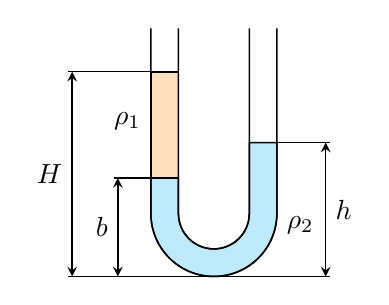
\begin{tikzpicture}[>=stealth,line width=.55pt]\draw[fill=cyan!25](0,1.2)--(0,.75) arc (180:360:.8)--(1.6,1.65)--(1.25,1.65)--(1.25,.75)arc(360:180:.45)--(.35,1.2)--cycle;\draw[fill=orange!25](0,1.2)rectangle(.35,2.55);\draw(0,3.1)--(0,.75)arc(180:360:.8)--(1.6,3.1) (.35,3.1)--(.35,.75)arc(180:360:.45)--(1.25,3.1);\node[left]at(0,1.92){$\rho_1$};\node[right]at(1.6,.6){$\rho_2$};\draw[<->](-1,-.05)--(-1,2.55)node[midway,left]{$H$};\draw[<->](-.42,-.05)--(-.42,1.2)node[midway,left]{$b$};\draw[<->](2.22,-.05)--(2.22,1.65)node[midway,right]{$h$};\draw[thin](-1.05,-.05)--(2.27,-.05) (-1.05,2.55)--(0,2.55) (-.47,1.2)--(0,1.2) (1.6,1.65)--(2.27,1.65);\end{tikzpicture}\end{center}В широкую U-образную трубку с вертикальными прямыми коленами налиты керосин и вода (см. рис.). На рисунке b  =  $10\,\text{см}$, H  =  $30\,\text{см}$. Какова высота жидкости в правом колене?
}{
\smallskip\noindent\textbf{Решение}\par
$1$.  Рассмотрим давление жидкостей в обоих коленах на уровне границы жидкостей. По закону Паскаля давление в обоих коленах на этом уровне должно быть одинаковым.
$2$.  Поскольку высота столба жидкости в левом колене больше, чем в правом, делаем вывод, что в левом колене плотность жидкости меньше, чем в правом, то есть в левом  — керосин, в правом  — вода. Давление жидкости в левом колене равно $p_1=\rho_1g ( H - b ) + p_a,$ в правом колене равно $p_2=\rho_2g ( h - b ) + p_a.$ Из равенства давлений получаем: 

\[h= \frac{\rho_1 ( H - b )}{\rho_2} + b= \frac{800 \cdot ( 30 - 10 )}{1000} + 10=26\,\text{см}.\]

Ответ: $26\,\text{см}$.
}

% Source 50822: https://phys-ege.sdamgia.ru/problem?id=50822
\BankTask{50822}{
Со дна озера, имеющего глубину H  =  $20\,\text{м}$, медленно поднимается пузырёк воздуха. Определите объём пузырька $V_{2}$ на расстоянии h  =  $1\,\text{м}$ от поверхности воды, если у дна озера пузырёк имел объём $V_{1}$  =  $1{,}1\,\text{мм}^{3}$. Давление воздуха на уровне поверхности воды равно нормальному атмосферному давлению. Силу поверхностного натяжения не учитывать, температуры воды в озере и воздуха в пузырьке считать постоянными.
}{
\smallskip\noindent\textbf{Решение}\par
Давление воздуха внутри пузырька равно внешнему давлению со стороны воды. Значит, давление воздуха в пузырьке в двух состояниях равны:

$p_1=\rho gH + p_a;$
$p_2=\rho gh + p_a.$

Так как температура воды в озере постоянна, то изменение объема воздуха в пузырьке происходит изотермически при неизменной массе. По закону Бойля  — Мариотта $p_1V_1=p_2V_2,$ откуда находим объем воздуха в пузырьке, находящемся у поверхности

\[V_2 = \frac{( \rho gH + p_a ) V_1}{\rho gh + p_a} = \frac{( 10 ^3 \cdot 10 \cdot 20 + 10 ^{5} ) \cdot 1{,}1}{10 ^3 \cdot 10 \cdot 1 + 10 ^{5}} =3\,\text{мм} ^3 .\]

Ответ: $3\,\text{мм}^{3}$.
}

% Source 30001: https://phys-ege.sdamgia.ru/problem?id=30001
\BankTask{30001}{
В запаянной с одного конца трубке находится влажный воздух, отделенный от атмосферы столбиком ртути длиной l  =  $76\,\text{мм}$. Когда трубка лежит горизонтально, относительная влажность воздуха $\varphi_1$ в ней равна $80$\%. Какой станет относительная влажность этого воздуха $\varphi_2,$ если трубку поставить вертикально, открытым концом вниз? Атмосферное давление равно $760\,\text{мм}$ рт. ст. Температуру считать постоянной.
}{
\smallskip\noindent\textbf{Решение}\par
$1$.  Относительная влажность воздуха в трубке в первом случае: $\varphi_1= \frac{p_1}{p_{\,\text{н}}} ,$ где $p_{1}$  — давление водяных паров в трубке, $p_{\,\text{н}}$  — давление насыщенных водяных паров при той же температуре. Для второго случая относительная влажность воздуха в трубке: $\varphi_2= \frac{p_2}{p_{\,\text{н}}} ,$ где $p_{2}$  — парциальное давление водяных паров в трубке.

\begin{center}\begin{tikzpicture}[task graph,>=stealth]\draw(.35,0)arc(-90:-270:.35)--(4.4,.7);\draw(.35,0)--(4.4,0);\draw(4.4,.35)ellipse(.16 and .43);\draw[fill=orange!30](1.62,0)rectangle(3.05,.7);\draw(0,-.1)--(0,-1.05)(1.62,0)--(1.62,-1.05)(3.05,0)--(3.05,-1.05);\draw[<->](0,-.88)--(1.62,-.88)node[midway,above]{\(l_1\)};\draw[<->](1.62,-.88)--(3.05,-.88)node[midway,above]{\(l\)};\node at(3.96,.95){\(p_0\)};\end{tikzpicture}\end{center}

\begin{center}\begin{tikzpicture}[task graph,>=stealth]\draw(0,0)--(0,3.55)arc(180:0:.33)--(.66,0);\draw(.33,0)ellipse(.44 and .15);\draw[fill=orange!30](0,1.26)rectangle(.66,2.48);\draw(.66,1.26)--(1.75,1.26)(.66,2.48)--(1.75,2.48)(.33,3.88)--(1.75,3.88);\draw[<->](1.59,1.26)--(1.59,2.48)node[midway,left]{\(l\)};\draw[<->](1.59,2.48)--(1.59,3.88)node[midway,left]{\(l_2\)};\node at(-.46,.4){\(p_0\)};\end{tikzpicture}\end{center}

$2$.  Давление влажного воздуха в первом случае равно атмосферному давлению: $p_1 \,\text{вл}=p_0,$ а во втором случае  — $p_2\,\text{вл}=p_0 - \rho g l,$ где \ensuremath{\rho} — плотность ртути, а l  — длина столбика ртути. Заметим, что $p_0=\rho g H,$ где H  =  $760\,\text{мм}$. 
$3$.  Объем влажного воздуха при изменении положения трубки изменился так, как изменились длины столбиков воздуха, запертых ртутью. Считаем влажный воздух идеальным газом. Поэтому по закону Бойля  — Мариотта можем записать:

\[\frac{V_2}{V_1} = \frac{l_2}{l_1} = \frac{p_0}{p_0 - \rho g l} .\]

$4$.  Из уравнения Клапейрона  — Менделеева следует, что: 

$p= \frac{\nu R T}{V} ,$ $p_{\,\text{вл}}= \frac{( \nu + \nu_{\,\text{св}} ) R T}{V} ,$

 где p  — парциальное давление водяного пара, $p_{\,\text{вл}}$  — давление влажного воздуха, $\nu$ — количество моль водяного пара в трубке, $\nu_{\,\text{св}}$  — количество моль сухого воздуха в трубке. Отсюда следует, что:

\[\frac{p}{p_{\,\text{вл}}} = \frac{\nu}{\nu + \nu_{\,\text{св}}} = const.\]

Поэтому $\frac{p_1}{p_2} = \frac{p_1 \,\text{вл}}{p_2 \,\text{вл}} ,$ и для изотермического процесса для парциальных давлений водяного пара имеем: 

\[\frac{p_1}{p_2} = \frac{V_2}{V_1} = \frac{p_0}{p_0 - \rho g l} .\]

$5$.  После объединения записанных выше уравнений получим выражение для относительной влажности воздуха во втором случае: 

\[\varphi_2=\varphi_1 \cdot \frac{p_0 - \rho g l}{p_0} =\varphi_1 \cdot \frac{\rho g H - \rho g l}{\rho g H} =\varphi_1 \frac{H - l}{H} =80 \cdot \frac{760 - 76}{760} =72 \%.\]

Ответ: $\varphi_2=72 \%.$
}

\end{document}
